\documentclass[../notesdecours.tex]{subfiles}

\begin{document}
\part{Formalisme de Dirac} \label{Formalisme de Dirac}
Dans la première section de ce cours traitant de la physique quantique, il a été mention de la mesure de la position d'une particule, de son impulsion, et que pour tout \textbf{état quantique}, les incertitudes liées à la position et à l'impulsion obéissent à une certaine relation : la relation d'incertitude de Heisenberg. Dans la deuxième section, nous établissons les principes fondamentaux de la physique quantique, et dérivons une équation qui tient compte de la dualité onde-corpuscule. En régime non-relativiste, il s'agit de l'équation de Schrödinger. Dans la troisième, nous résolvons cette équation, qui est une équation d'onde, et introduisons donc une fonction solution, que nous appelons \textbf{fonction d'onde}. Une fonction d'onde décrit donc une particule quantique. \\

Dans ces sections, nous n'avons pas défini rigoureusement ce que nous entendons par "état quantique", et n'avons pas caractérisé les fonctions d'onde en termes de continuité, dérivabilité, domaine de définiton, etc. C'est tout le sujet de cette partie : \textbf{formaliser cette nouvelle physique}. \\

Nous allons tout d'abord commencer par décrire les fonctions d'onde à l'aide de notions d'Analyse. Ensuite, nous introduisons le \textbf{formalisme de Dirac} qui sert à décrire et manipuler les \textbf{états quantiques}.
\section{Expérience de Stern-Gerlach}
L'expérience de Stern-Gerlach (1922) consistait à faire passer des atomes d'argent dans un champ magnétique non uniforme (fig \ref{fig:chap4-sterngerlach}). Classiquement, les atomes d'argent, ayant un moment cinétique et un moment magnétique orbital également nul, ne devraient pas subir l'influence du champ magnétique. L'expérience montre que le faisceau se \textbf{sépare en deux}. Ce résultat, inexpliqué par la compréhension "classique" de la matière, a trouvé une explication en physique quantique, avec l'introduction du moment cinétique de spin.\\

\begin{figure}[h]
\centering
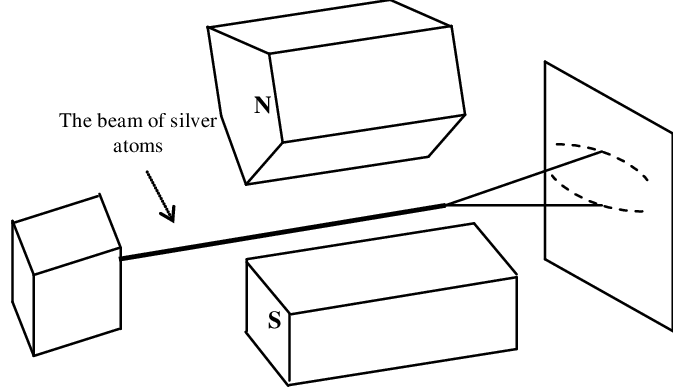
\includegraphics[width=0.5\linewidth]{Stern-Gerlach}
\caption{Dispositif expérimental de l'\href{https://fr.wikipedia.org/wiki/Expérience_de_Stern_et_Gerlach}{expérience de Stern-Gerlach (\textit{lien cliquable})}}
\label{fig:chap4-sterngerlach}
\end{figure}

Mathématiquement, rappelons à toute fin utile que:
\begin{align}
\text{Moment angulaire } \bm{L} &= m\bm{r}\ti\bm{v} \label{Moment angulaire}\\
\text{Moment magnétique } m &= I\norm{\bm{S}}	= \frac{ev}{2\pi r} \pi r^2 = \frac{1}{2}evr = \frac{1}{2}\frac{e}{m}L	&I = \frac{ev}{2\pi r}\\
\bm{m} &= \frac{1}{2}\frac{e}{m}\bm{L} \label{moment magnétique}
\end{align}
Où I est le courant et $\bm{S}$ est la surface considérée.\\

En pratique, les atomes/particules élémentaires suivent cette relation à un facteur prêt : $\bm{m} = \frac{g}{2}\frac{e}{m}\bm{L}$, où $g$ est le \textbf{facteur de Londé}. Elle prend différentes valeurs en fonction de ce que nous considérons: nous avons $g = -2.002$ pour un électron, $g_n = -3.8$ et $g_p = 5.6$.\\

En pratique, nous mettrons en évidence la quantification du moment angulaire en mesurant le moment magnétique. L'énergie d'un moment magnétique dans un champ magnétique sera donnée par l'expression
\begin{equation}
E = \bm{m}\cdot\bm{B}
\end{equation}
Lorsque le champ est non-uniforme, nous observons un gradient d'énergie:
\begin{equation}
\bm{F} = \bm{\nabla}\cdot(\bm{m}\cdot\bm{B}) = \bm{\nabla}\cdot(E)
\end{equation}
En faisant l'expérience, nous nous attendons donc à observer ce gradient d'énergie - et donc un "gradient de résultats". Ce n'est pas le cas: seul deux tâches sont observées. Chaque électron se comporte comme un aimant à seulement deux directions vertiables possibles: Nord-Sud ou Sud-Nord. Cette propriété quantique s'appelle le spin, et s'écrit:
\begin{equation}
S = \pm \frac{\h}{2}
\end{equation}

\begin{center}
\begin{figure}[h]
\centering
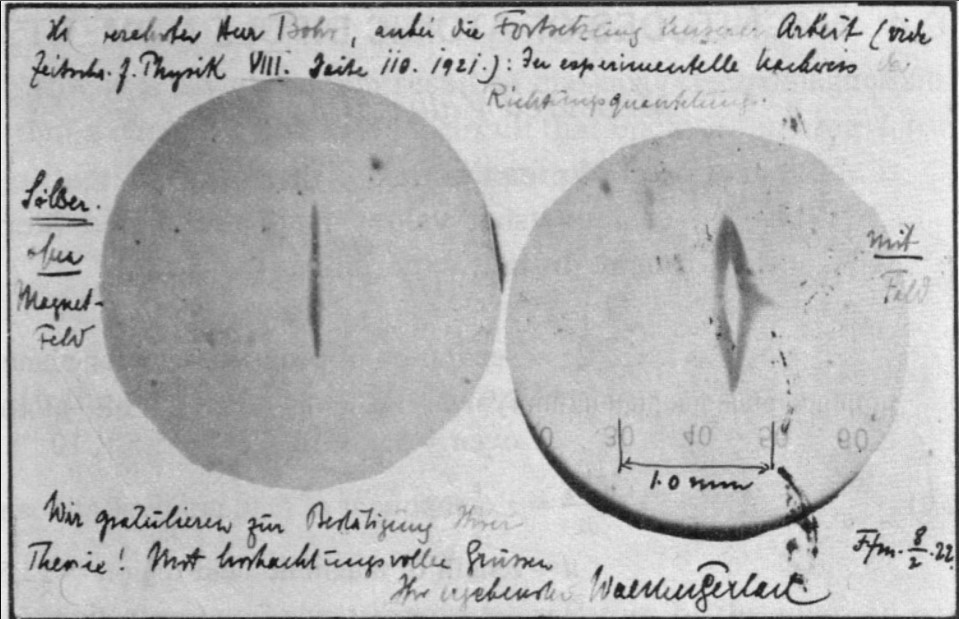
\includegraphics[width=0.50\textwidth]{exp.png}
\caption{Une photo des rayons séparés, avec un message. La traduction donne: "Ci-contre, une preuve expérimentale du spin quantique. Nous vous félicitons pour la vérification expérimentale de votre théorie".}
\end{figure}
\end{center}
\newpage
\section{Espace mathématique des fonctions d'onde}
\label{Espace mathématique des fonctions d'onde}
\begin{center}
\textit{La section actuelle ne figure pas dans les notes de Prof. Massar. Elles sont tirées de l'ouvrage de référence.}
\end{center}
Jusqu'à présent, nous avons mentionné les fonctions d'onde à plusieurs reprises sans nous être définis un \textbf{espace de fonctions} auxquelles elles appartiennent. Or c'est un objet mathématique, il ne faudrait pas commettre trop de pêchés sans connaître sa nature (même si on est physicien). Nous savons qu'une fonction d'onde doit respecter 

$$ \int_{\mathbb R ^3} |\psi(\bm{r}, t)| ^2 \; \d ^3 \bm{r} = 1 \; ,$$
donc nous nous savons déjà qu'elle doit être de carré sommable.
$$\psi \in L^2$$
L'espace des fonctions de carré sommable est bien trop vaste. Pour décrire des quantités physiques, nous voulons de notre fonction qu'elle soit également continue et infiniment dérivable (afin de ne pas rencontrer de discontinuités à très petite échelle). Nous nommons $\mathcal F$ l'espace ainsi obtenu. Cet espace, des fonctions de carré sommable, continues et infiniment dérivables, contient les fonctions partout définies (une particule dans le vide) comme les fonctions à support borné (une particule dans un laboratoire). Nous notons alors $\psi \in \mathcal{F}$.
$$\psi \in \mathcal{F} \subset L^2$$

\subsection{Structure de $\mathcal{F}$}
\begin{itemize}
\item L'\textit{espace des fonctions} (c'est la terminologie que nous utiliserons pour $\mathcal F$) est un \textbf{espace vectoriel}. \\
\item Un produit scalaire $(\cdot, \cdot)$ est défini sur $\mathcal F$.
\begin{equation}
\forall \varphi, \psi \in \mathcal F : \quad (\varphi, \psi)\;   \doteq \int_{\mathbb R ^3} \varphi ^\star(\bm{r}) \psi(\bm{r}) \; \d ^3 r
\label{Produit scalaire - Espace des fonctions d'onde}
\end{equation}
$(\varphi,\psi)$ est le produit scalaire de $\psi(\bm{r})$ par $\varphi(\bm{r})$ : elle converge toujours si $\varphi$ et $\psi$ appartiennent à $\mathcal{F}$.\\

Le produit scalaire est \textbf{sesquilinéaire}, et vérifie une égalité similaire à celle de Cauchy-Schwarz : 
$$ \forall \varphi_1, \varphi_2 \; : \; (\varphi_1, \varphi_2) \leq \sqrt{(\varphi_1, \varphi_1)}\sqrt{(\varphi_2, \varphi_2)} \; .$$

Ci-contre, une série de propriétés découlant de $\ref{Produit scalaire - Espace des fonctions d'onde}$:
\begin{align*}
(\varphi,\psi) &= (\psi,\varphi)^*\\
(\varphi,\lambda_1\psi_1 + \lambda_2\psi_2) &= \lambda_1 (\varphi,\psi_1) + \lambda_2 (\varphi,\psi_2)\\
(\lambda_1\varphi_1 + \lambda_2\varphi_2,\psi) &= \lambda_1^* (\varphi_1,\psi) + \lambda_2^* (\varphi_2,\psi)
\end{align*}
Le produit scalaire est \emph{linéaire} par rapport à la seconde fonction du couple, et \emph{anti-linéaire} par rapport à la première.
\end{itemize}

\subsection{Opérateurs linéaires pour $\mathcal F$}
Nous pouvons parler des opérateurs linéaires qui agissent sur des fonctions de $\mathcal F$. $A$ est un tel opérateur si et seulement si $$\forall \varphi \in \mathcal F \; : \; A\varphi = \psi \quad \in 
\mathcal F$$
Soient $A$ et $B$ deux tels opérateurs. Alors, nous pouvons les prendre en produit et définir un troisième opérateur $AB$ défini comme suit :
$$AB : \mathcal F \rightarrow \mathcal F : \varphi \longmapsto A[B(\varphi)]\; .$$
Similairement, nous pouvons définir
$$BA : \mathcal F \rightarrow \mathcal F : \varphi \longmapsto B[A(\varphi)]\; ,$$
et si nous faisons ça c'est parce qu'en général, $AB \neq BA$ : on dit que les opérateurs ne \textbf{commutent pas}. On en profite pour définir un troisième opérateur, qui lui, prend deux opérateurs et vérifie s'ils commutent :
$$[\cdot, \cdot] : A, B \longmapsto AB-BA$$
et on appelle cet opérateur \textbf{commutateur de $A$ et de $B$}.

\subsection{Bases orthonormées discrètes dans $\mathcal F$}
\subsubsection{Base ? Orthonormée ?}
Continuons dans notre lancée matheuse ! Après avoir parlé de structure, d'opérateurs, parlons de base. Soit une base de $\mathcal F$, $\{u_i(\bm{r})\}$. Par définition, 
\begin{equation}
\label{eq:base_orthonormee_F}
\forall \varphi \in \mathcal F \; : \quad \exists \{c_i\}_{i=1, ...} \; \mathrm{t.q} \quad \varphi(\bm{r}) = \sum_i c_i u_i(\bm{r}) \; ,
\end{equation}
où les coefficients $c_i$ sont dits qu'ils \textit{représentent} $\varphi$ dans la base $\{u_i(\bm{r})\}$.\\

La base est orthonormée pourvu que 
\begin{equation}
\label{eq:orthonorm_F}
(u_i, u_j) = \int_{\mathbb R ^3} u_i ^\star(\bm{r}) u_j(\bm{r}) \; \d ^3 \bm{r} = \delta_{ij} \; .
\end{equation}

Avec la représentation de toute fonction dans la base, nous pouvons réécrire le produit scalaire entre des fonctions $\varphi$ et $\psi$ représentés par des coefficients $b_i$ et $c_i$ comme :
$$(\varphi, \psi) = \sum_i b_i ^\star c_i$$
Ceci a pour implication directe 
\begin{equation}
\label{eq:base_orthonormee_coeffsci}
(\psi, \psi) = \sum_i |c_i|^2
\end{equation}

\subsubsection{Relation de fermeture}
La \textit{relation de fermeture} exprime que $\{u_i(\bm{r})\}$ est une base. Elle sera d'application pour vérifier à partir d'un ensemble de fonctions qu'elles forment bien une base de $\mathcal F$.

$$\{u_i(\bm{r})\} \; \text{est une base} \; \iff \forall \psi \in \mathcal F, \;\text{on a }$$
\begin{eqnarray}
\psi(\bm{r}) &=& \sum_i (u_i, \psi) u_i(r) \\
&=& \sum_i \left[\int_{\mathbb R ^3} u_i ^\star(\bm{r}') \psi(\bm{r}') \; \d ^3 \bm{r}'\right] u_i(\bm{r}) \\
&=& \int_{\mathbb R ^3}\d ^3  \underbrace{\left[\sum_iu_i ^\star(\bm{r}')u_i(\bm{r}) \right]}_{G(\bm{r}, \bm{r}')}\psi(\bm{r}') \\
&=& \int_{\mathbb R ^3}\d ^3 G(\bm{r}, \bm{r}')\psi(\bm{r}') \\
&\iff& G(\bm{r}, \bm{r}') = \delta(\bm{r}-\bm{r}') \\
&\iff& \sum_iu_i ^\star(\bm{r}')u_i(\bm{r}) = \delta(\bm{r}-\bm{r}') 
\end{eqnarray}
La dernière égalité est la \textbf{relation de fermeture}. Nous pouvons alors montrer que toute fonction $\psi(\bm{r})$ quelconque peut s'écrire sous la forme
\begin{equation}
\psi(\bm{r}) = \int d^3r' \; \psi(\bm{r}') \delta (\bm{r} - \bm{r}')
\label{implication relation de fermeture}
\end{equation}
\subsection{Généralisation de la notion de base}
En mécanique quantique, il existe des bases qui n'appartiennent \textbf{pas} à $\mathcal F$, sur lesquelles il est tout de même important de compter pour développer des fonctions d'onde. Voici une série d'exemples particulièrement importants.
\subsubsection{L'exemple des ondes planes}
\paragraph{Un produit scalaire}
L'espace des ondes planes,
$$\left\{ v_p(x) = e^{ipx/\h}\right\}\; ,$$
n'est pas de carré sommable. Par contre, si nous commettons un pêché et écrivons un produit scalaire (à une constante près) entre une fonction $\psi$ de $\mathcal F$ et un $v_p$ comme s'il était dans $\mathcal F$ (soyons fous!) :
$$(\psi, v_p) = \dfrac{1}{\sqrt{2\pi\h}} \int_{\mathbb R}\d x \; \psi(x) e^{-ipx/\h}$$
Nous voyons que si nous définissons une fonction de $p$ pour l'égalité ci-dessus, notre pêché se serait résumé en une Transformée de Fourier de $\psi$, soit quelque chose qui existe\footnote{C'est beau d'être physicien. On fait n'importe quoi tant que ça marche, et ça sera au matheux de vérifier.} ! Ceci motive à considérer notre ensemble d'ondes planes comme une base et de considérer la Transformée de Fourier comme un produit scalaire avec un $v_p$.
$$\bar{\psi}(p) = \dfrac{1}{\sqrt{2\pi\h}} \int_{\mathbb R}\d x \; \psi(x) e^{-ipx/\h}$$
\paragraph{Des composantes}
D'autre part, nous pouvons interpréter la transformée inverse
$$\psi(x) = \dfrac{1}{\sqrt{2\pi\h}} \int_{\mathbb R}\d p \; \bar\psi(p) e^{ipx/\h}$$
comme l'expression de $\psi$ dans la base des $v_p$, avec comme composantes $\bar \psi(p)$, l'équivalent des $c_i$ de l'équation \eqref{eq:base_orthonormee_F}. \\

Par l'identité de Parseval, nous avons aussi l'équivalent de la relation \eqref{eq:base_orthonormee_coeffsci} :
$$(\psi, \psi) = \int_{\mathbb R} |\bar \psi(p)|^2 \; \d p$$
\paragraph{Une relation d'orthonormalisation}
Avec la relation (cf. livre de référence) 
$$\dfrac{1}{2\pi} = \int_{\mathbb R} \d k e^{iku} = \delta(u) \; ,$$
nous pouvons obtenir une relation qui ressemble à une belle relation d'orthonormalisation :
$$(v_p, v_{p'}) = ... = \delta(p-p')$$
En comparant à \eqref{eq:orthonorm_F}, nous avons ici des indices continus, et avant on avait des indices discrets. Attention, ici, lorsque $p = p'$, nous n'avons pas $1$ : ça diverge. On dit que $v_p$ et $v_{p'}$ sont \textbf{orthonormés au sens de Dirac}. \\

Cet exemple des ondes planes motive l'extension du concept de base à des objets qui ne sont pas dans $\mathcal{F}$.
\subsubsection{L'exemple des fonctions delta}
Soit $\bm{r_0} = (x_0,y_0,z_0)$. On intrduit un ensemble de fonctions définies par $\zeta_{r_0} (\bm{r}) = \delta(r-r_0)$. L'ensemble $\{\zeta_{r_0}(\bm{r})\}$ est la base des fonctions delta centrées en un point $\bm{r}_0$ ; $\zeta_{r_0} (\bm{r})$ n'étant pas de carré sommable, nous avons que $\zeta_{r_0} (\bm{r}) \notin \mathcal{F}$.\\

Nous pouvons alors réécrire la relation $\eqref{implication relation de fermeture}$ sous la forme
\begin{align}
\psi (\bm{r}) &= \int d^3r_0 \; \psi(\bm{r}_0)\zeta_{r_0} (\bm{r})\\
\psi (\bm{r}_0) &= \int d^3r \; \zeta_{\bm{r}_0}^* \psi(\bm{r})
\end{align}

\subsubsection{Notion générale de base "orthonormée" continue}
Une base orthonormée continue sera un ensemble de fonctions qui ont les propriétés suivantes.
\begin{enumerate}
\item Il s'agit d'un ensemble de fonctions $\{ w_\alpha(\bm{r})\}$ repérées par un indice continu. \\

\item Les fonctions satisfont une \textbf{relation d'orthonormalisation} :
$$(w_{\alpha}, w_{\alpha'}) \doteq \int w_{\alpha}(\bm{r})^\star w_{\alpha'}(\bm{r}) = \delta(w_{\alpha} - w_{\alpha'})$$

\item Les fonctions satisfont une \textbf{relation de fermeture} :
$$\int w_{\alpha}(\bm{r})^\star w_{\alpha}(\bm{r}') = \delta(\bm{r}-\bm{r}')$$
\end{enumerate}
\section{Notations propre à la Mécanique Quantique}
Dans le cadre de la Mécanique Quantique, nous nous placerons dans des expaces de Hilbert $\mathbb{H}$ séparables. Un espace de Hilbert est un espace pré-hilbertien (c'est-à-dire, muni d'un produit scalaire hermitien) dans lequel toute suite de Cauchy converge. \\

Nous introduisons:
\begin{itemize}
\item Vecteur $\in \mathbb{H}$ : $\ket{\psi}$. Il s'agit d'un vecteur colonne $v$, appelé le ket.
\item Vecteur transposé conjugué $\in \mathbb{H}$ : $\bra{\psi}$. Il s'agit du vecteur ligne\footnote{Nous pouvons également le voir comme un élément du dual $\mathbb{H}^*$} $\overline{v}^T$, appelé le bra.
\item Le produit scalaire $\braket{\varphi,\psi}$, appelé le braket.
\end{itemize}
\subsection{Correspondance entre bra et ket}
Si $\ket{\psi} = \alpha \ket{\Phi} + \beta\ket{\Phi'}$, alors $\bra{\psi} = \overline{\alpha}\bra{\Phi}+\overline{\beta}\bra{\Phi'}$ : la correspondance bra $\rightarrow$ ket est donc antilinéaire. 
\begin{remark} Si $\lambda$ est un nombre complexe et $\ket{\psi}$ un ket, alors $\lambda\ket{\psi}$ est un ket. Nous l'écrirons parfois $\ket{\lambda\psi}$. Il faudra alors faire attention que la relation entre bra et ket étant anti-linéaire, $\bra{\lambda\psi} = \overline{\lambda}\ket{\psi}$. \end{remark}

Notons que les états quantiques sont:
\begin{enumerate}
\item \emph{normalisés}:
\begin{equation}
\braket{\psi|\psi} = 1
\end{equation}
en raison de l'interprétation probabiliste.
\item \emph{définis à une phrase prêt}:
\begin{align}
&\ket{\psi} 	&e^{i\varphi}\ket{\psi}
\end{align}
représentent le même état quantique.
\end{enumerate}
Nous sommes dans un espace projectif de Hilbert. Dès lors,

\begin{center}
\begin{tabular}{ c c c } 
$\ket{\psi} \thicksim \ket{\varphi}$ & quand & $\ket{\psi} = \lambda\ket{\varphi}$  
\end{tabular}
\end{center}

\subsubsection{Exemples}
\textbf{Spin $\frac{1}{2}$}: base orthonormée = \bigg\{$\ket{\uparrow}$,$\ket{\downarrow}$\bigg\}.\\

Nous pouvons définir un état arbitraire:
\begin{equation}
\ket{\psi} = \cos\frac{\theta}{2} \ket{\uparrow}+e^{i\varphi}\sin\frac{\theta}{2}\ket{\downarrow}
\end{equation}
Où $\theta\in[0,\pi]$ et $\varphi \in [0,2\pi]$ et $\theta,\varphi$ appartiennent à la sphère de Bloch.\\

Si $\ket{\varphi} = \cos\frac{\theta'}{2}\ket{\uparrow}+e^{i\varphi'}\sin\frac{\theta'}{2}\ket{\downarrow}$, alors le produit scalaire donnera
\begin{equation}
\braket{\varphi|\psi} = \cos\frac{\theta}{2}\cos\frac{\cos'}{2}+e^{\varphi-\varphi'}\sin\frac{\theta}{2}\sin\frac{\theta'}{2}
\end{equation}

\textbf{Oscillateur harmonique:} base orthonormée = $\bigg\{\ket{n} : n=0,1,2,...\bigg\}$ et les états d'énergies sont donnés par $E_n = \h\omega\bigg\{n+\frac{1}{2}\bigg\}$.\\

Nous pouvons définir un état arbitraire par $\ket{\psi} = \sum_n c_n \ket{n}$ avec $\sum_n \norm{c_n}^2 = 1$.

\section{Opérateurs linéaires}
Soit $A : \mathbb{H} \rightarrow \mathbb{H} : \ket{\psi} \rightarrow A\ket{\psi}$ un opérateur linéaire, c'est à dire tel quel $A(a\ket{\psi}+b\ket{\varphi}) = a(A\ket{\psi})+b(A\ket{\varphi})$. Soit $B$ un (autre) isomorphisme\footnote{Demander vérification à Massar.} sur le même ensemble $\mathbb{H}$. Nous pouvons définir plusieurs opérations:
\begin{itemize}
\item \textbf{Produit d'opérateurs}: $(AB)\ket{\psi} = A(B\ket{\psi})$. B agit d'abord sur ket $\ket{\psi}$ pour donner $B\ket{\psi}$, et A agira ensuite sur $A\ket{\psi}$.
\item En général, $AB\neq BA$, le commutateur [A,B] de A,B est par définition [A,B] = AB-BA.
\item \textbf{Anticommutateur} : $\bigg\{A,B\bigg\} = AB+BA$.
\end{itemize}
Action de A sur le dual/les bras. Soit $A: \mathbb{H}^* \rightarrow \mathbb{H}^* : \bra{\varphi} \rightarrow \bra{\varphi}A$ est défini par $\Big\{\bra{\varphi}A\Big\}\ket{\psi} = \bra{\varphi}\Big\{A\ket{\psi}\Big\}$, pour tout$\ket{\varphi},\ket{\psi}$. Nous le noterons $\braket{\varphi|A|\psi}$.
\begin{remark} Observons que l'ordre dans lequel apparaît les symbols a une importance capital. Seul les nombres complexes peuvent être déplacés sans influencer le résultat. \end{remark}

\begin{exemple} 
Soit $\ket{\psi}$ et $\ket{\Theta}$ deux kets. Ecrivons les dans l'ordre inverse: $\bra{\psi}$ et $\bra{\Theta}$. Considérons 
\begin{equation}
\ket{\psi}\bra{\Theta}
\label{ket bra}
\end{equation}
Prenons un ket $\ket{\gamma}$ tel que
\begin{equation}
\ket{\psi}\braket{\Theta|\gamma}
\end{equation}
Nous avons que $\braket{\Theta|\gamma}$ est un nombre complexe ; par conséquent, nous avons que un bra $\bra{\psi}$ multiplié par un scalaire. Nous avons alors que $\eqref{ket bra}$ appliqué à un ket donne un nouveau ket.
\end{exemple}

\section{Opérateur adjoint $A^\dag$}
\begin{definition} Soit $A$: $\mathbb{H} \rightarrow \mathbb{H}$ un opérateur linéaire. Nous définissons l'opérateur adjoint $A^\dag : \mathbb{H} \rightarrow \mathbb{H}$ par $\braket{\psi|A^\dag|\varphi} = \braket{\varphi|A|\psi}^*$ pour tout $\ket{\psi},\ket{\varphi}$. \end{definition}

Si $\big\{\ket{u_i}\big\}$ forme une base orthonormée, alors:
\begin{itemize}
\item $\braket{u_i|A|u_j} = a_{ij}$
\item $\braket{u_i|A^\dag|u_j} = a^*_{ij}$
\end{itemize}
$\rightarrow A^\dag = \overline{A^T}$ est la transposée conjuguée\footnote{Ask teacher what's up.}.\\
\subsection{Propriétés intéressantes}
Nous donnons ici une série de propriétés de l'opérateur adjoint $A^\dag$.
\begin{center}
\fbox{\begin{minipage}{7cm}
\begin{enumerate}
\item $(A^\dag)^\dag = A$
\item $(\lambda A)^\dag = \lambda^*A^\dag$ pour tout $\lambda\in\mathbb{C}$.
\item $(A+B)^\dag = A^\dag + B^\dag$
\item $(AB)^\dag = A^\dag B^\dag$.
\item Si $A = \ket{\alpha}\bra{\beta}$, alors $A^\dag = \ket{\beta}\bra{\alpha}$.
\end{enumerate}
\end{minipage}}
\end{center}

\subsection{Exemples d'opérateurs}
\begin{enumerate}
\item Soit $A=\ket{\alpha}\bra{\beta}$. Alors,
\begin{align}
\braket{\varphi|A|\psi} &= \braket{\varphi|\Big\{\ket{\alpha}\bra{\beta}\Big\}|\psi}\\
&= \braket{\varphi|\alpha}\braket{\beta|\psi}\\
\text{Et } A\ket{\psi} &= \ket{\alpha}\braket{\beta|\psi}
\end{align}
\item Soit $\Big\{(u_i)\Big\}$ une base orthonormée. Nous avons que $\braket{u_i|u_j} = \delta_{ij}$. De plus, nous appelons \emph{éléments de la matrice A} l'opérateur
\begin{equation}
\braket{u_i|A|u_j} = a_{ij}
\end{equation}
Nous pouvons représenter A dans la base via
\begin{equation}
A = \sum_{i,j} a_{ij} \ket{u_i}\bra{u_j}
\end{equation}
\end{enumerate}

\section{Opérateur Hermitien et observable}
\begin{definition}
Un opérateur $A$ est \emph{Hermitien} (ou encore Hermitique) lorsque $A = A^\dag$.
\end{definition}
\begin{Property}
En particulier, nous avons alors que $\braket{u_i|A|u_j} = a_{ij} = \braket{u_i|A^\dag|u_j} = \overline{a_{ji}}$.
\end{Property}
\begin{definition}
Un opérateur Hermitien est dit observable lorsqu'il possède une base de vecteurs propres.
\end{definition}


\subsection{Equation aux vecteurs propres}
Soit 
\begin{equation}
A\ket{\psi} = \lambda\ket{\psi}.
\end{equation}
\begin{Property}
Lorsque $A=A^\dag$ est Hermitien, les valeurs propres sont réelles.
\end{Property}
\begin{proof}
$\lambda = \braket{\psi|A|\psi} = \braket{\psi|A^\dag|\psi} = \overline{\braket{\psi|A|\psi}} = \overline{\lambda}$.
\end{proof}
\begin{Property}
Lorsqu'un opérateur est Hermitien, alors les vecteurs propres associés à des valeurs propres distinctes sont orthogonaux.
\begin{align}
A\ket{\psi} &= \lambda\ket{\psi}		&A\ket{\Phi} = \lambda'\ket{\Phi}
\end{align}
\end{Property}
\begin{proof}
\begin{align*}
\lambda\braket{\Phi|\psi} &= \bra{\Phi}(A\ket{\psi}) = \braket{\Phi|A^\dag|\psi} = \braket{\psi|A|\Phi}^*\\
&= \bra{\psi}(\lambda'\ket{\Phi})^* = \lambda'^* \braket{\psi|\Phi}^* = \lambda' \braket{\Phi|\psi}
\end{align*}
Nous avons en général que $\lambda - \lambda' \neq 0$. Dès lors, il s'ensuit que $\braket{\Phi|\psi} = 0$ : la conclusion s'ensuit.
\end{proof}
\begin{Property}
Pour un opérateur Hermitien $A$, nous avons que:
\begin{itemize}
\item En dimension finie, $A$ possède une base orthonormée de vecteurs propres.
\item En dimension infinie, cela n'est pas nécessairement le cas.
\end{itemize}
\end{Property}
\begin{proof}
Cette propriété n'est pas démontrée. Pour une preuve détaillée, se référer aux notes 2019-2020 de MATH-F102 (\emph{second quadrimestre}) par Samuel FIORINI.
\end{proof}

\subsection{Exemples d'opérateurs}
\begin{itemize}
\item \underline{\textbf{Projecteurs}} : Soit un opérateur $\pi$ tel que: $\begin{cases} 
\pi = \pi^\dag\\
\pi^2 = \pi
\end{cases}$. Les valeurs propres sont alors soit 0, soit 1.
\begin{proof}
\begin{align*}
\pi\ket{\psi} &= \lambda\ket{\psi}\\
\lambda\braket{\psi|\psi} &= \braket{\psi|\pi|\psi} = \braket{\psi|\pi^2|\psi}\\
&= (\bra{\psi}\pi)(\pi\ket{\psi})\\
&= \lambda \overline{\lambda} \braket{\psi|\psi}		&\lambda\in\mathbb{R}\\
\end{align*}
Dès lors, nous avons que $\lambda^2 = \lambda$ : soit donc $\lambda = 0$ ou $\lambda = 1$.
\end{proof}

Nous avons alors que $\ket{\psi}$ et $\bra{\psi}$ sont des projecteurs $\forall\ket{\psi}$.\\

\begin{remark}
Une application linéaire $\psi$ tel que $\psi^2 = \psi$ est dite idempotente. \end{remark}

\begin{definition} Si $\Big\{\ket{u_i}: i\in\mathbb{N} \Big\}$ est une base orthonomée et si I est un sous-ensemble de $\mathbb{N}$, alors $\pi = \sum_{i\in I} \ket{u_i}\bra{u_i}$ est un projecteur. \end{definition}

\item \underline{\textbf{Oscillateur harmonique}} : Soit $\Big\{\ket{n}: n\in\mathbb{N} \Big\}$. Nous définissons alors plusieurs opérations:
	\begin{itemize}
	\item[$\blacksquare$] Opérateur destruction: $a\ket{n} = \sqrt{n}\ket{n-1}$ et $a\ket{0} = 0$. En particulier, les éléments de la matrice de a sont donnés par $\braket{m|a|n} = \sqrt{n}\delta_{m}^{n-1}$.
	\item[$\blacksquare$] Opérateur création: Soit $a^\dag$ l'hermitien conjugué de $a$. Nous avons alors que $a^\dag\ket{n} = \sqrt{n+1}\ket{n+1}$.
	\end{itemize}
\item \underline{\textbf{Opérateur identité}}: Soit $\mathbb{I}\ket{\psi} = \ket{\psi}$ pour tout $\ket{\psi}$ sur une base orthonormée $\Big\{\ket{u_i}: n\in\mathbb{N} \Big\}$. Alors, nous avons que $\mathbb{I} = \sum_i \ket{u_i}\bra{u_i}$. Il s'agit de la définition de l'opérateur identité.
\item \underline{\textbf{Spin $\frac{1}{2}$}}: Soit une base orthonormée \bigg\{$\ket{\uparrow}$,$\ket{\downarrow}$\bigg\}.
\end{itemize}


\newpage
\part{Postulats de la Mécanique Quantique}
\label{Postulats de la Mecanique Quantique}
Dans ce chapitre, nous allons énoncer les postulats de la mécanique quantique selon le formalisme développé en \ref{Formalisme de Dirac}. Ils permettront de répondre aux questions suivantes:
\begin{enumerate}
\item Comment décrire mathématiquement l'état d'un système quantique à un instant donné?
\item Comment, cet état étant donné, prévoir les résultats de mesure des diverses grandeurs physiques?
\item Comment trouver l'état du système à un instant t quelconque lorsqu'on connait  ce état à l'instant $t_0$?
\end{enumerate}
\section{Énoncé des postulats}

\begin{center}
\fbox{\begin{minipage}{15cm}
\begin{center}
\textbf{PREMIER POSTULAT - Vecteur d'état $\ket{\psi}$}
\end{center}
A tout système quantique correspond au moins un $\emph{espace de }\mathcal{H}ilbert$ complexe et séparable $\mathbb{H}$ dans lequel la théorie quantique du système peut-être formulée. Tout état accessible du système quantique correspond alors à un \emph{vecteur normé $\ket{\psi}$} dans $\mathcal{H}$ dont la phase globale est arbitraire. 
\end{minipage}}
\end{center}
Ce postulat a plusieurs implications:
\begin{itemize}
\item Tout système quantique est placé dans un esapce vectoriel : cela implique un \textit{principe de superposition}. De fait, si $\ket{\psi_1 (t)}$ et $\ket{\psi_2 (t)}$ sont des vecteurs d'états, alors $\alpha \ket{\psi_1 (t)} + \beta\ket{\psi_2 (t)}$ est également un vecteur d'état.
\item Le produit scalaire $\braket{\psi|\varphi}$ est sesquilinéaire. Nous pouvons alors effectuer des calculs d'angles et de distances dans $\mathcal{H}$.
\item Un état du système est bien défini \textit{séparément} des grandeurs observables, celles-ci modifiant son état.
\end{itemize}


\begin{center}
\fbox{\begin{minipage}{15cm}
\begin{center}
\textbf{SECOND POSTULAT - Observables $\ket{\hat{P}}$}
\end{center}
A toute grandeur classique correspond un \emph{opérateur hermitien} $\hat{P}$ agissant dans $\mathcal{H}$. Le processus de mesure quantique consiste à relever les propriétés fondamentales de ces opérateurs. En d'autres termes, les résultats de la mesure d'une obserable sont les diverses valeurs propres (réelles) de cette observable.
\end{minipage}}
\end{center}
Lorsque l'opérateur $A$ possède une base de vecteurs propres, nous pouvons écrire $A$ sous la forme\begin{equation}
A = \sum_n a_nP_n
\end{equation}
où $a_n$ est une valeur propre de A et $P_n$ est un projecteur sur le sous-espace propre de $A$ de la valeur propre $a_n$.\\

La probabilité d'observer le résultat $a_n$ dans l'état $\ket{\psi}$ est donnée par $P(a_n) = \braket{\psi|P_n|\psi}$ où $P_n$ est un projecteur.\\

Nous pouvons vérifier que cela respecte bien les axiomes de la théorie des probabilités:
\begin{enumerate}
\item \textbf{Normalisation}: $\sum_n P(a_n) = \sum_n \braket{\psi|P_n|\psi} = \braket{\psi|\sum_n P_n|\psi} = \braket{\psi|\mathbb{I}|\psi} = \braket{\psi|\psi} = 1.$
\item \textbf{Positivité}: $P(a_n) = \braket{\psi|P_n|\psi} = \braket{\psi|P_n^2|\psi} = \norm{P_n\ket{\psi}}^2 \geq 0.$
\item \textbf{Probabilité indépendante de la phase}. En effet, lorsque $\ket{\psi}\to e^{i\varphi}\ket{\psi}$, $P(a_n)$ ne change pas.
\end{enumerate}

\begin{center}
\fbox{\begin{minipage}{15cm}
\begin{center}
\textbf{TROISIEME POSTULAT - Interprétation probabiliste}
\end{center}
Le résultat d'une mesure sur un opérateur $\hat{A}$ à un instant donné est aléatoire. Si ce résultat est une valeur propre $a$, la probabilité d'obtenir précisément cette valeur propre plutôt qu'une autre dans le spectre de $\hat{A}$ est donnée par le module carré de la projection de l'état sur l'état propre $\ket{a}$ associé à la valeur propre mesurée.
\label{Postulat3}
\end{minipage}}
\end{center}
\begin{itemize}
\item Nous ne sommes en mesure que d'effectuer des prédictions probabilistes. Il faut dès lors effectuer un grand nombre d'expériences. Nous n'avons accès qu'aux \emph{valeurs moyennes} de $\hat{A}$, et les écart-types associés.
\item Le Théorème d'Heinsenberg $\Delta A\Delta B \geq \frac{\norm{{[\hat{A},\hat{B}]}}}{2}$ implique que deux observables qui ne commutent pas ne peuvent pas être observées en même temps.
\item \textit{Règle de Born} (spectre discret) : La probabilité de transition entre les états $\ket{\psi}$ et $\ket{\varphi}$ est donnée par $P_\varphi = \norm{\braket{\varphi|\psi}}^2$ lorsque le spectre est discret non-dégénéré.

\item \textit{Règle de Born} (spectre continu) : La probabilité $dP(\alpha)$ d'obtenir un résultat entre $\alpha$ et $\alpha+d\alpha$ est donnée par $dP = \norm{\braket{u_\alpha|\psi}}^2d\alpha$.
\end{itemize}

\subsection{Valeur moyenne d'une observable $\mathcal{\hat{A}}$}

\begin{definition}
	La moyenne $\braket{\hat{\mathcal{A}}}$ d'une observable $\mathcal{\hat{A}}$ par rapport à un état $\ket{\psi}$ est donnée par
	\begin{align}
		\braket{A} &= \sum_n a_n P(a_n) = \sum_n a_n \braket{\psi|P_n|\psi} = \braket{\psi|\sum_n a_n P_n | \psi} & \braket{A} &= \braket{\psi|A|\psi}
	\end{align}
\end{definition}

\subsection{Ecart quadratique moyen}
\begin{lemma}
$A^2 = \sum_n a_n^2P_n$
\end{lemma}
\begin{proof}
\begin{equation*}
A^2 = (\sum_n a_nP_n)(\sum_{n'} a_nP_n) = \sum_{nn'} a_na_{n'}P_nP_{n} = \sum_n a_n^2P_n.
\end{equation*}
Effectivement, remarquons que $P_nP_{n'}$ revient à $\delta_{nn'}P_n'$.
\end{proof}

\begin{Property}
	L'incertitude d'une observable $\mathcal{\hat{A}}$ est donnée par
	\begin{equation}
		\Delta \hat{A} = \sqrt{\braket{\psi|A^2|\psi} - \braket{\psi|A|\psi}^2}
	\end{equation}
\end{Property}
\begin{proof}
	\begin{align*}
		\Delta A^2 &= \sum_n a_n^2 P(a_n) - \langle A\rangle^2\\
		&= \sum_n a_n^2 \braket{\psi|P_n|\psi} - \langle A\rangle^2\\
		&= \sum_n a_n^2 \braket{\psi|P_n|\psi} - \langle A\rangle^2\\
		&= \braket{\psi|\sum_n a_n^2 P_n|\psi} - \langle A\rangle^2\\
		&= \braket{\psi|A^2|\psi} - \braket{\psi|A|\psi}^2.
		\end{align*}	
\end{proof}

\begin{remark} Nous ne pouvons pas mesurer simultanément des obserbables qui ne commutent pas. A l'inverse, nous \textbf{pouvons} mesurer simultanément des observables qui commutent: $[A,B] = 0$. Ceci constitue une réécriture et généralisation du principe d'incertitude d'Heinsenberg \eqref{Heinsenberg}.\end{remark}

\begin{center}
\fbox{\begin{minipage}{15cm}
\begin{center}
\textbf{QUATRIEME POSTULAT - Postulat de la mesure}
\end{center}
Si la mesure de l'observable $\hat{A}$ sur le système dans l'état $\ket{\psi}$ fournit une valeur propre $\lambda$ (associée au vecteur propre $\ket{\lambda}$), l'état du système immédiatement après la mesure est \emph{projeté} sur le sous-espace propre associé à $\lambda$.
\end{minipage}}
\end{center}

\begin{itemize}
\item La mesure de $\ket{\psi} \rightarrow \hat{P}\ket{\psi} \propto \ket{\lambda}$ s'effectue au moyen d'un projetcteur orthogonal $\hat{P}^2 = \hat{P}$, $\hat{P}^\dagger = \hat{P}$.
\item C'est un processus \textit{irréversible} qui ne conserve pas la probabilité. Après une mesure, on parle de "perte de la cohérence quantique".
\item Aux échelles microscopiques, toute mesure perturbe fortement le système (exemple: Effet Compton). 
\end{itemize}

\subsection{Evolution des systèmes dans le temps}
\label{Postulat 5}
\begin{center}
\fbox{\begin{minipage}{15cm}
\begin{center}
\textbf{CINQUIEME POSTULAT - Évolution des États}
\end{center}
A tout système peut-être associé un opérateur hermitien $\hat{H}$ appelé Hamiltonien et représentant l'énergie totale du système. Cet opérateur régit l'évolution temporelle du vecteur d'état $\ket{\psi (t,\bm{x})}$ au moyen de l'équation de Schrödinger
\begin{equation*}
i\h \frac{d}{dt} \ket{\psi(t,\bm{x})} = \hat{H}\ket{\psi (t,\bm{x})}
\end{equation*}
\end{minipage}}
\end{center}
\begin{itemize}
\item L'évolution est \textit{unitaire}, c'est à dire que $\ket{\psi (t,\bm{x})} = \hat{U} (t,t_0)\ket{\psi (t_0,\bm{x})}$ par conservation de la probabilité.
\item Un état stationnaire est un état propre de l'hamiltonien. 
\item Dans un potentiel stationnaire, l'évolution des états s'écrit
\begin{equation}
	U(t,t_0) = e^{-i\omega t} = e^{-\frac{i}{\h}Et}
\end{equation}
comme nous l'explique l'équation \eqref{Evolution des états}.
\end{itemize}
Soit une base $\Big\{\ket{u_i}\Big\}$ orthonormée. Alors,
\begin{align}
\ket{\psi(t)} &= \sum_i c_i(t)\ket{u_i}\\
H(t) &= \sum_{i i'} \ket{u_i}\bra{u_{i'}} H_{ii'} (t)
\end{align}

\begin{Property} Soit $\ket{\psi(t)}$ une solution de l'équation de Schrödinger $\eqref{Schrodinger}$. Alors, le produit scalaire $\braket{\psi(t)|\psi(t)}$ est constante. \end{Property}
\begin{proof}
\begin{equation}
\frac{d}{dt} \braket{\psi(t)|\psi(t)} = (\frac{d}{dt}\bra{\psi(t)})\ket{\psi(t)} + \bra{\psi(t)}(\frac{d}{dt}\ket{\psi(t)})
\end{equation}
Remarquons que $H$ est un opérateur hamiltonien. Dès lors,
\begin{align}
\bra{\psi(t)}H &= -i\frac{d}{dt}\bra{\psi(t)}		&H^\dag = H.
\end{align}
Dès lors,
\begin{align}
\frac{d}{dt} \braket{\psi(t)|\psi(t)} = i \braket{\psi(t) | H(t) | \psi(t)} - i \braket{\psi(t)|H(t)|\psi(t)} = 0.
\end{align}
\end{proof}

\begin{remark} Nous prenons $\braket{\psi(t)|\psi(t)} = 1.$ \end{remark}

\subsection{Réduction du paquet d'onde}
Supposons que nous souhaitions mesurer, en un instant $t$ donné, une grandeur physique $\mathcal{A}$. Si nous connaissons $\ket{\psi}$, nous pouvons\footnote{à travers des techniques qui seront expliquées ultérieurement.} obtenir les probabilité des différents résultats possibles. Cependant, en effectuant l'expérience, nous n'obtiendront qu'un seul des résultats possible: ce faisant après avoir obtenu le résultat $a_n$\footnote{on parle de la valeur propre $a_n$.}, on postule que l'état du sytème change: $\ket{\psi} \to \ket{u_n}$.

\begin{center}
\fbox{\begin{minipage}{15cm}
\begin{center}
\textbf{SIXIEME POSTULAT - Réduction du paquet d'onde}
\end{center}
Si la mesure de la grandeur physique A, à l'instant t, sur un système représenté par le vecteur $\ket{\psi}$ donne comme résultat la valeur propre $a_n$, alors l'état du système immédiatement après la mesure est projecté sur le sous-espace propre associé à $a_n$.
\begin{equation*}
\ket{\psi'} = \frac{\hat{P}_n\ket{\psi}}{\sqrt{P(a_n)}}
\end{equation*}
Où $P(a_n)$ est la probabilité de trouver comme résultat la valeur propre $a_n$, et $\hat{P}_n$ est l'opérateur projecteur défini par $\hat{P}_n = \sum_{k=1}^{g_n} \ket{u_{n,k}}\bra{u_{n,k}}$, où $g_n$ est le degré de dégénérescence de la valeur propre $a_n$ et les $\ket{u_{n,k}}$ sont les vecteurs de son sous-espace propre.
\end{minipage}}
\end{center}


\subsection{Hamiltonien indépendant du temps}
Lorsque l'Hamiltonien ne dépend pas du temps, nous parlons de système \emph{conservatif}. Rappelons l'équation aux valeurs propres $\eqref{kikoo}$:
\begin{equation*}
H\ket{\varphi_{n,\tau}} = E_n \ket{\varphi_{n,\tau}}
\end{equation*}
Où les $\ket{\varphi_{n,\tau}}$ forment une base de vecteurs propres (H est une observable). En particulier, notons que H étant hermitique, cette dernière égalité peut se réécrire:
\begin{equation}
\bra{\varphi_{n,\tau}}H = E_n \bra{\varphi_{n,\tau}}
\end{equation}
Nous allons montrer que $E_n$ et $\ket{\varphi_{n,\tau}}$ suffisent à déterminer les solutions de l'équation de Schrödinger.\\

Notons que $\ket{\varphi_{n,\tau}}$ formant une base, nous pouvons pour chaque valeur de t développer un état du système $\ket{\psi}$ dans la base:
\begin{equation}
\ket{\psi (t)} = \sum_{n,\tau} c_{n,\tau} (t)\ket{\varphi_{n,\tau}}
\end{equation}
Où $c_{n,\tau}(t) = \braket{\varphi_{n,\tau}|\psi (t)}$. Projetons alors l'équation de Schrödinger sur chacun des états $\ket{\varphi_{n,\tau}}$. Nous obtenons que:
\begin{align*}
i\h\frac{\partial}{\partial t}\braket{\varphi_{n,\tau}|\psi (t)} &= \braket{\varphi_{n,\tau} | H | \psi (t)}\\
i\h\partial_tc_{n,\tau}(t) &= E_n \braket{\varphi_{n,\tau}|\psi(t)} = E_nc_{n,\tau}
\end{align*}
Nous obtenons alors l'équation différentielle d'ordre 1 en $c_{n,\tau} (t)$
\begin{equation}
i\h\partial_tc_{n,\tau}(t) = E_nc_{n,\tau}.
\end{equation}
Sa solution générale est donné par 
\begin{equation}
c_{n,\tau} (t) = c_{n,\tau} (t_0) e^{-i \frac{E_n}{\h} (t-t_0)}
\end{equation}
Dès lors, le vecteur d'état $\ket{\psi(t)}$ vaudra
\begin{equation}
\ket{\psi(t)} = \sum_n c_n(t_0)e^{-i\frac{E_n}{\h}(t-t_0)} \ket{\varphi_{n,\tau}}
\end{equation}

Pour résoudre l'équation de Schrödinger avec un Hamiltonien indépendant du temps, il suffit de \underline{diagonaliser} l'Hamiltonien et de connaitre la \underline{décomposition} de $\ket{\psi}$ à l'instant initial dans la base des vecteurs propres de $\mathcal{H}$.\\

\begin{remark}
	Nous venons de dériver un résultat obtenu précédemment, précisement dans la discussion autour de l'équation \eqref{Evolution des états}.
\end{remark}

\subsection{Opérateurs unitaires}
La notion d'unité est introduite en $\ref{AppendeiceA}$ ; plus spécifiquement en les définitions \ref{Unitaire} et en \ref{Hermitienne}. En utilisant les notations introduites dans en \ref{Formalisme de Dirac}, nous pouvons réécrire cela sous la forme
\begin{align}
U^{-1} &= U^\dag\\
UU^\dag &= U^\dag U = \mathbb{I}
\end{align}
\begin{Property} Soit U une application unitaire. Soient $\ket{\psi}$, $\ket{\varphi}$ deux kets. Notons
\begin{align*}
\ket{\tilde{\psi}} &= U\ket{\psi}\\
\ket{\tilde{\varphi}} &= U\ket{\varphi}.
\end{align*}
Alors, le produit scalaire est conservé:
\begin{equation}
\braket{\tilde{\psi}|\tilde{\psi}} = \braket{\psi|\varphi}.
\end{equation}
\end{Property}

\begin{Property} 
Soit $\{\ket{i}\}$ une base orthonormée et U une matrice unitaire. Alors, $\{U\ket{i}\} = \ket{i}\}$ est également une base orthonormée et 
\begin{equation}
\ket{\tilde{i}} = U\ket{i} = \sum_j \ket{j}\bra{j}U\ket{i} = \sum_j \ket{j}U_{ji}
\end{equation}
est la matrice de changement de base.
\end{Property}

\begin{Property}
Si U et V sont des matrices unitaires, alors UV est unitaire. \end{Property}

\begin{Property} Si U est unitaire et $\ket{\psi}$ est un vecteur propre de U
\begin{align}
U\ket{\psi} &= \lambda\ket{\psi}		&\rightarrow \norm{\lambda}^2 = 1.
\end{align}
De plus, $\lambda = e^{i\varphi}$. Nous pouvons diagonaliser une matrice unitaire 
\begin{equation}
U = \sum_j e^{i\varphi_j}\ket{i}\bra{j}
\end{equation}
Où $\{\ket{j}\}$ est une base orthonormée de vecteurs propres. \end{Property}

\begin{theorem}
Si U est une matrice $n\ti n$ telle que $\braket{\psi|U^\dag U|\psi} = \braket{\psi|\psi}$ pour tout $\ket{\psi}$, alors U est unitaire\footnote{La matrice U appartient à $U_n$, l'ensemble des matrices de taille $n\ti n$ définie en \ref{Unitaire}} et donc $U^\dag U = \mathbb{I}$.
\end{theorem}
\begin{proof}
En utilisant le premier postulat de la Mécanique Quantique, nous pouvons écrire tout état sous la forme $\ket{\psi} = \ket{\alpha} + e^{i\varphi}\ket{\beta}$. Dès lors,
\begin{align*}
\braket{\psi|U^\dag U|\psi} &= \braket{\psi|\psi}\\
(\ket{\alpha} + e^{-i\varphi}\ket{\beta})(U^\dag U)(\ket{\alpha} + e^{i\varphi}\ket{\beta}) &= (\ket{\alpha} + e^{-i\varphi}\ket{\beta})(\ket{\alpha} + e^{i\varphi}\ket{\beta})\\
\braket{\alpha|U^\dag U|\alpha} + e^{-i\varphi}\braket{\beta|U^\dag U|\alpha} + e^{i\varphi}\braket{\alpha|U^\dag U|\beta} + \braket{\beta|U^\dag U|\beta} &= \braket{\alpha|\alpha} + e^{-i\varphi}\braket{\beta|\alpha} + e^{i\varphi}\braket{\alpha|\beta} + \braket{\beta|\beta}
\end{align*}
Or, nous avons que
\begin{align*}
\braket{\alpha|U^\dag U|\alpha} &= \braket{\alpha|\alpha}		&\braket{\beta|U^\dag U|\beta} = \braket{\beta|\beta}.
\end{align*}
Dès lors, 
\begin{align*}
\braket{\beta|U^\dag U |\alpha} &= \braket{\beta|\alpha}	&\forall\ket{\alpha}\ket{\beta},\\
\braket{\alpha|U^\dag U|\beta} &= \braket{\alpha|\beta}	&\forall\ket{\alpha}\ket{\beta}.
\end{align*}
Ce qui implique alors que $U^\dag U = \mathbb{I}$.
\end{proof}

\begin{Property} Si $\ket{\psi}$ est une solution de l'équation de Schrödinger, alors il existe un opérateur linéaire $U(t,t_0)$ tel que
\begin{equation}
\ket{\psi (t,t_0)} = U(t,t_0)\ket{\psi(t_0)}.
\end{equation} \label{1}\end{Property}

En utilisant ce résultat, nous obtenons que
\begin{align*}
i\partial_t U(t,t_0)\ket{\psi(t_0)} &= H(t)U(t,t_0)\ket{\psi(t_0)}		&\forall\ket{\psi(t_0)}\\
i\partial_t U(t,t_0) &= H(t)U(t,t_0)
\end{align*}
Avec la condition initiale $U(t_0,t_0) = \mathbb{I}$.\\

\begin{Property} Comme $\braket{\psi(t_0)|\psi(t)}$ est indépendant de t, il s'ensuit que 
\begin{align}
\braket{\psi(t_0)|U^\dag (t,t_0)U(t,t_0)|\psi(t_0)} &= \braket{\psi(t_0)|\psi(t_0)}		&\forall\ket{\psi(t_0)}.
\end{align}
Nous avons alors que $U(t,t_0)$ est une matrice unitaire. \end{Property}

\section{Fonction d'Opérateurs/de matrices}
Soit f: $\begin{pmatrix}
\mathbb{C} & \rightarrow & \mathbb{C}\\
x & \rightarrow & \sum_{n = 0}^{\infty} c_nx^n
\end{pmatrix}$ une fonction qui peut-être représentée par une série. Soit $A\in\mathbb{C}^{N\times N}$ une matrice. Alors on étend f à une fonction sur les matrices par
\begin{equation}
f: \begin{pmatrix}
\mathbb{C}^{N\times N} & \rightarrow & \mathbb{C}^{N\times N}\\
A & \rightarrow & \lim_{K\to\infty} \sum_{n = 0}^{k} c_n A^n
\end{pmatrix}
\end{equation}
lorsque cette limite existe.

\begin{Property} Si V est une matrice inversible $VV^{-1} = V^{-1}V = \mathbb{I}$, alors $f(V^{-1}AV) = V^{-1}f(A)V$ \end{Property}
\begin{proof}
\begin{align*}
f(V^{-1}AV) = \sum_{n = 0}^{\infty} c_n (V^{-1}AV)^n = \sum_{n = 0}^{\infty} c_n V^{-1} A^n V = V^{-1}f(A)V
\end{align*}
\end{proof}

\begin{Property}
Si D est une matrice diagonale $D = \begin{pmatrix}
\lambda_1 & 0 & ... & 0\\
0 & \lambda_2 & ... & 0\\
0 & 0 & ... & \lambda_N
\end{pmatrix}$, est $f(D)$ est diagonale et $f(D) = \begin{pmatrix}
f(\lambda_1) & 0 & ... & 0\\
0 & f(\lambda_2) & ... & 0\\
0 & 0 & ... & f(\lambda_N)
\end{pmatrix}$.
\end{Property}
\begin{lemma} Si A est une matrice diagonalisale, alors il existe V inversible tel que $V^{-1}AV = D$ est diagonal. Alors, $f(A) = V^{-1}f(D)V$. \end{lemma}
\begin{lemma} Si A est hermitien $A=A^\dag$, alors il existe V unitaire $U^{-1} = U^\dag$ tel que $A = U^{\dag}DU$ où $D$ est diagonal réel. Alors, $f(A) = U^{\dag}f(D)U$. \end{lemma}

\begin{remark} En notation de Dirac, $A = \sum_j a_j \ket{j}\bra{j}$ et $f(A) = \sum_j f(a_j) \ket{j}\bra{j}$. \end{remark}
\end{document}
